% !TEX TS-program = pdflatex
% !TEX encoding = UTF-8 Unicode
% !TEX root = ../main.tex
% !TEX spellcheck = en-US
% ****************************************************************************************
% File: results.tex
% Author: Jakob Spindler
% Date: 2024-10-16
% ****************************************************************************************
\chapter{Results}
\label{chapter:results}
The following chapter presents the results of the conducted emissions of the buck converter after the implementation of the afforementioned methods.

\section{Rail to Rail X-Cap}
\label{section:x_cap} 
A \qty{22}{\micro\farad} low ESL low ESR Capacitor (C7) is placed between the rails of the buck converter \autocite{885012209006WurthElektronik}.

\begin{figure}[htbp]
    \centering
    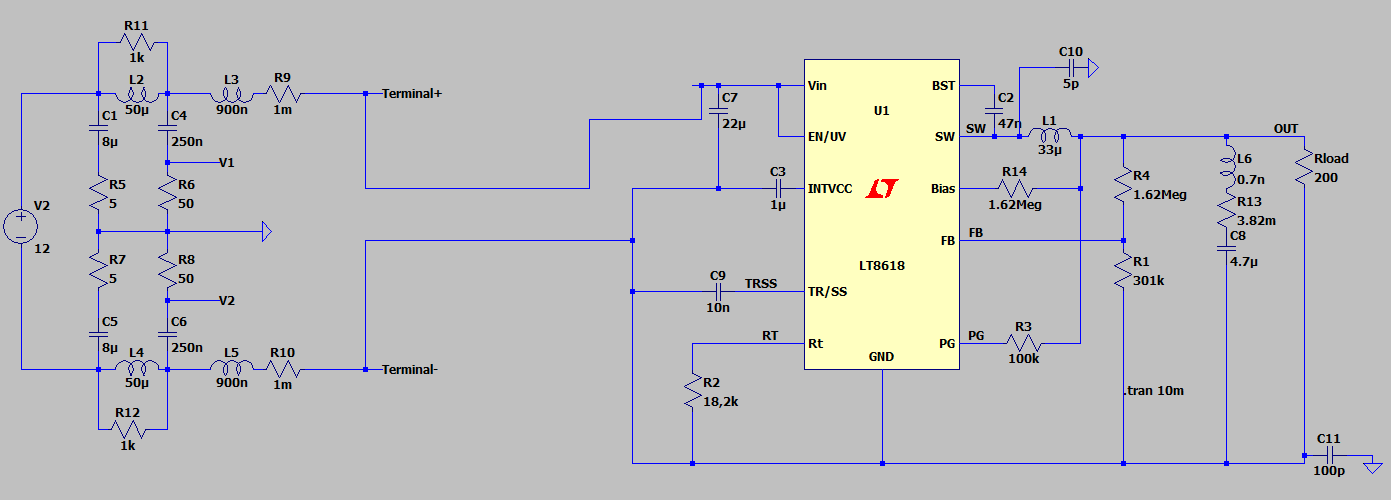
\includegraphics[width=0.8\textwidth]{img/schematic_no_cmc_22u_x_cap.png}
    \caption{Schematic: \GLS{acr:lisn} and buck converter with a rail to rail x-cap}
    \label{fig:x_cap_schematic}
\end{figure}

\begin{figure}[htbp]
    \centering
    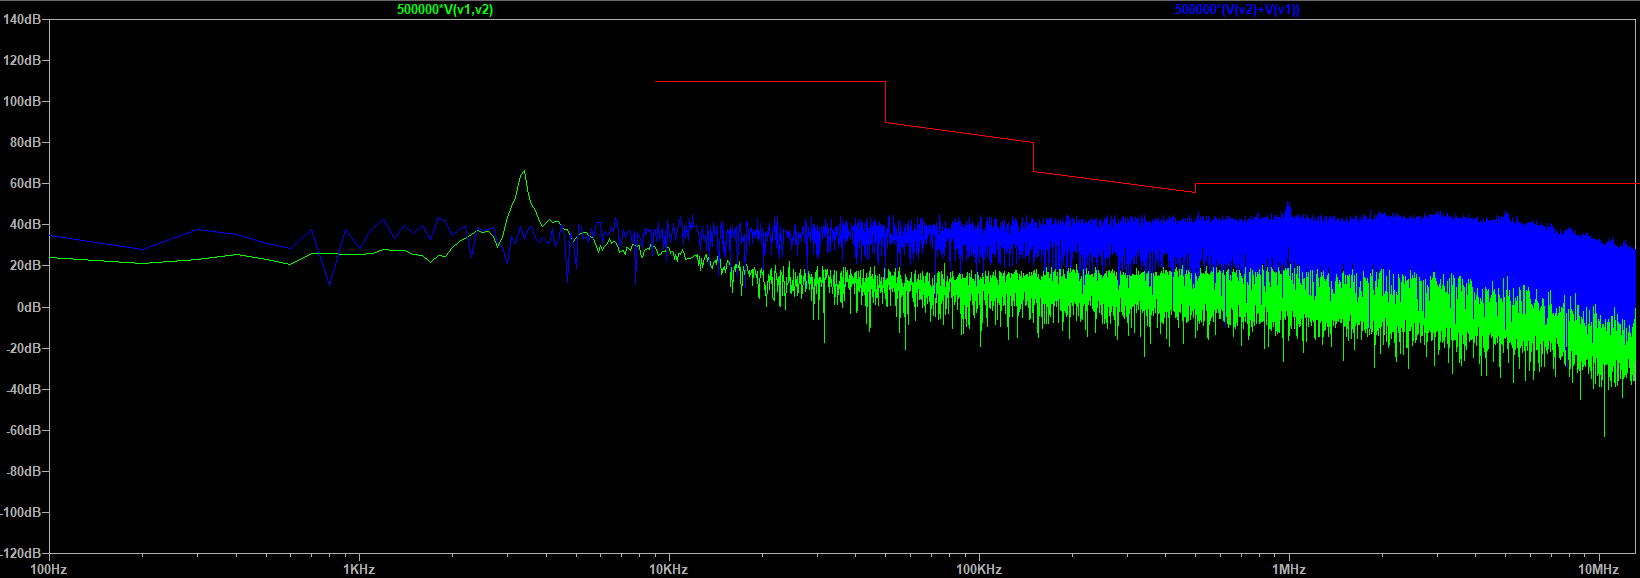
\includegraphics[width=0.8\textwidth]{img/emi_no_cmc_22u_x_cap.png}
    \caption{Conducted emissions of the buck converter with a rail to rail x-cap with \GLS{acr:dm} in green and \GLS{acr:cm} in blue, red line represents the conducted emissions limit}
    \label{fig:x_cap_emc}
\end{figure}

\begin{figure}
    \centering
    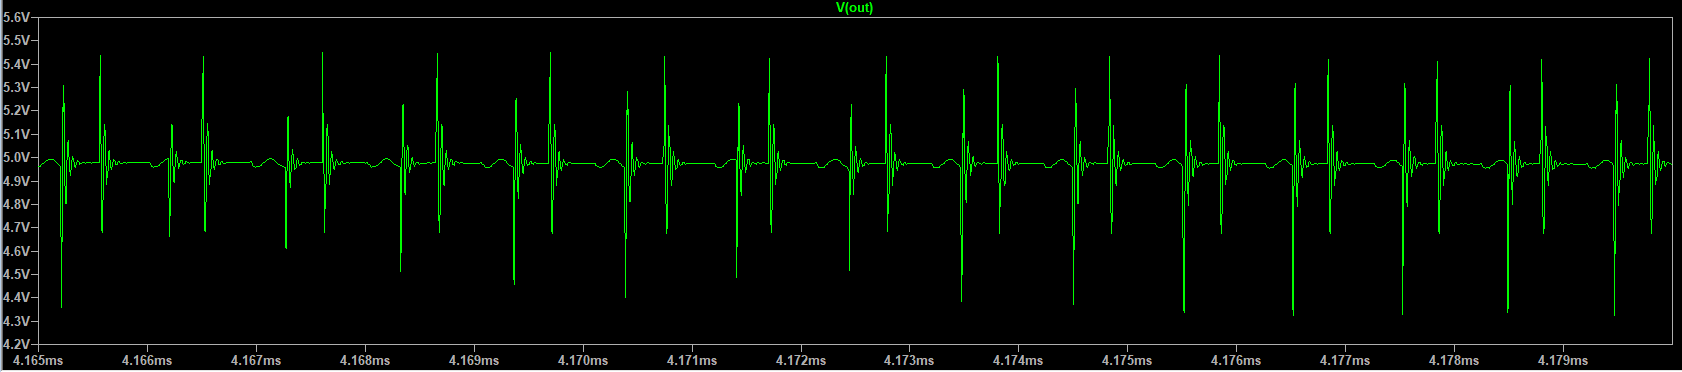
\includegraphics[width=0.8\textwidth]{ripple_22u_x_cap.png}
    \caption{steady state output voltage ripple of the buck converter with a rail to rail x-cap}
    \label{fig:x_cap_ripple}
\end{figure}

\section{Common Mode Choke and X-Cap}
\label{section:cmc_x_cap}
Additionally to the C7 X-Cap a \qty{250}{\micro\henry} common mode choke (L7) is placed on the rails \autocite{744235251WurthElektronik}.

\begin{figure}[htbp]
    \centering
    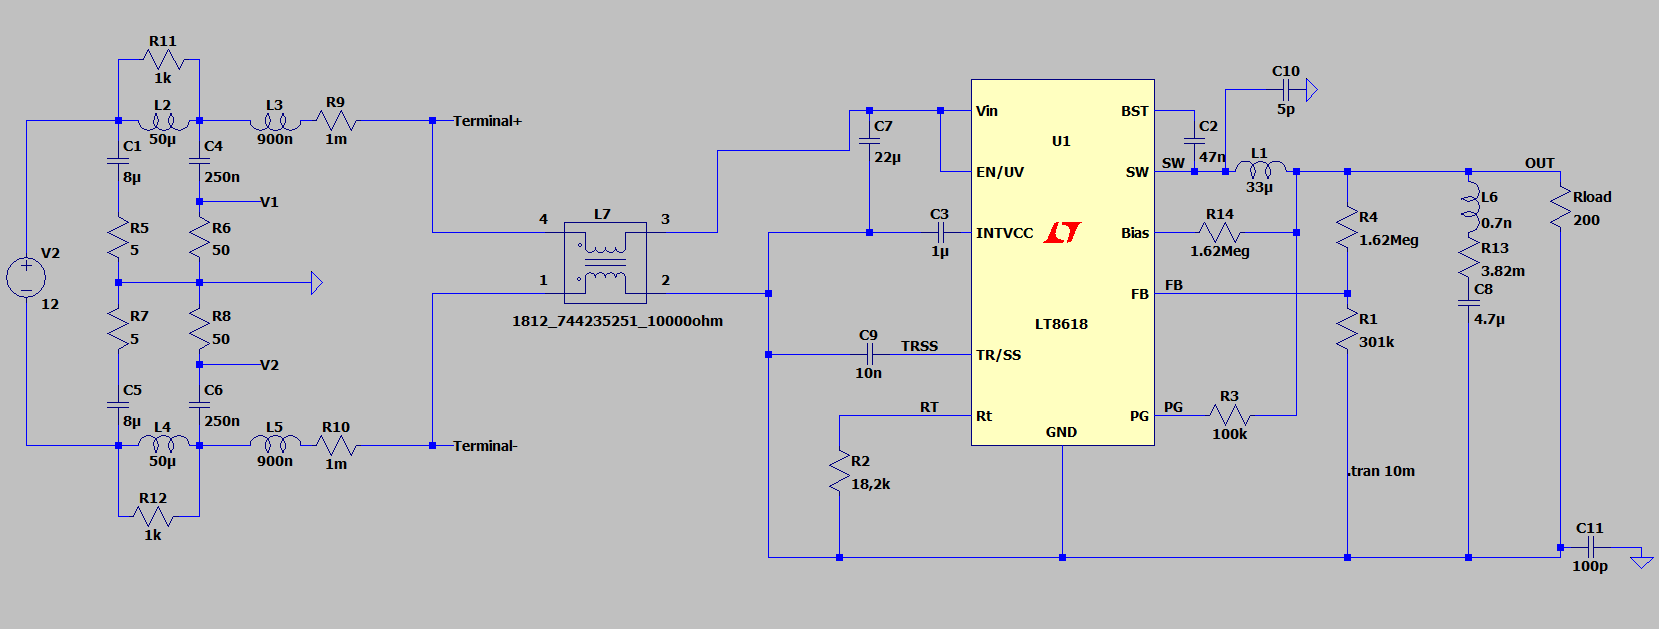
\includegraphics[width=0.8\textwidth]{img/schematic_cmc_22u_x_cap.png}
    \caption{Schematic: \GLS{acr:lisn} and buck converter with a rail to rail x-cap and a common mode choke}
    \label{fig:cmc_x_cap_schematic}
\end{figure}

\begin{figure}[htbp]
    \centering
    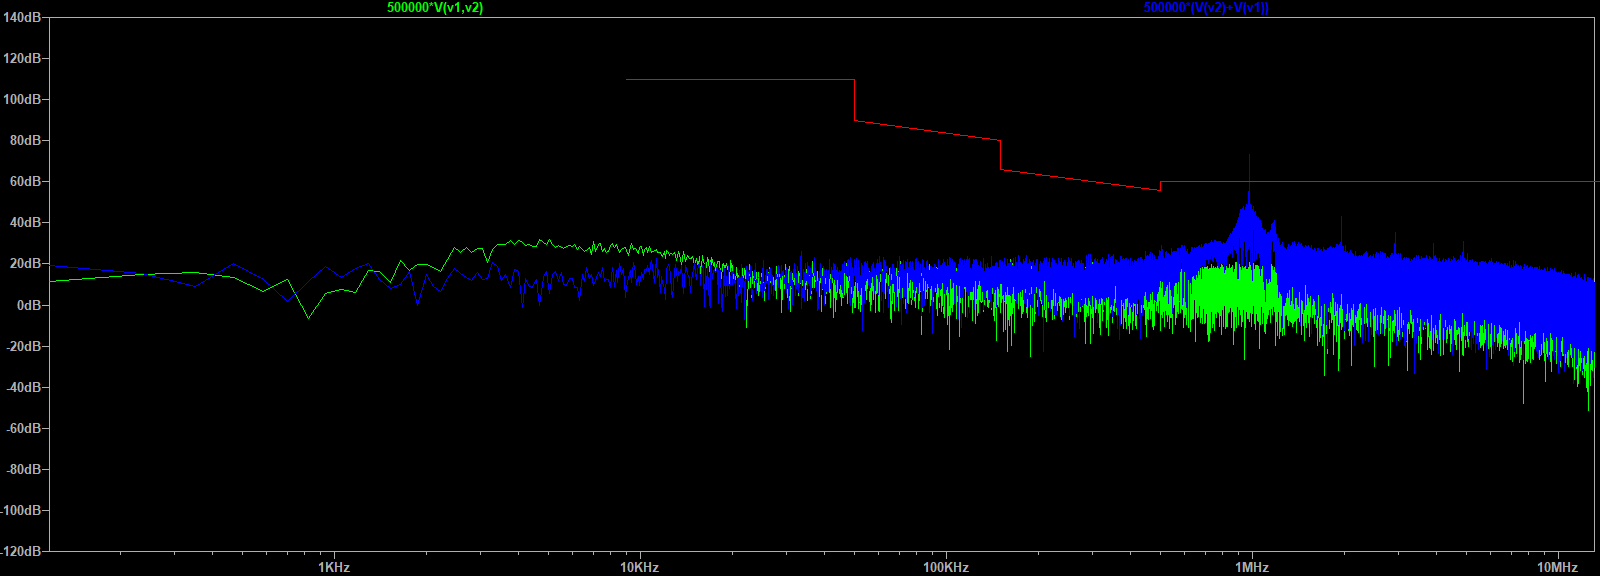
\includegraphics[width=0.8\textwidth]{img/emi_cmc_22u_x_cap.png}
    \caption{Conducted emissions of the buck converter with a rail to rail x-cap and a common mode choke with \GLS{acr:dm} in green and \GLS{acr:cm} in blue, red line represents the conducted emissions limit}
    \label{fig:cmc_x_cap_emc}
\end{figure}

\newpage

\section{Common Mode Choke, X-Cap and Y-Caps}
\label{section:cmc_x_cap_y_cap}

In addition to the C7 X-Cap and the L7 Common Mode Choke, \qty{10}{\nano\farad} Y-Caps (C12, C13) are placed between the rails and ground.

\begin{figure}[htbp]
    \centering
    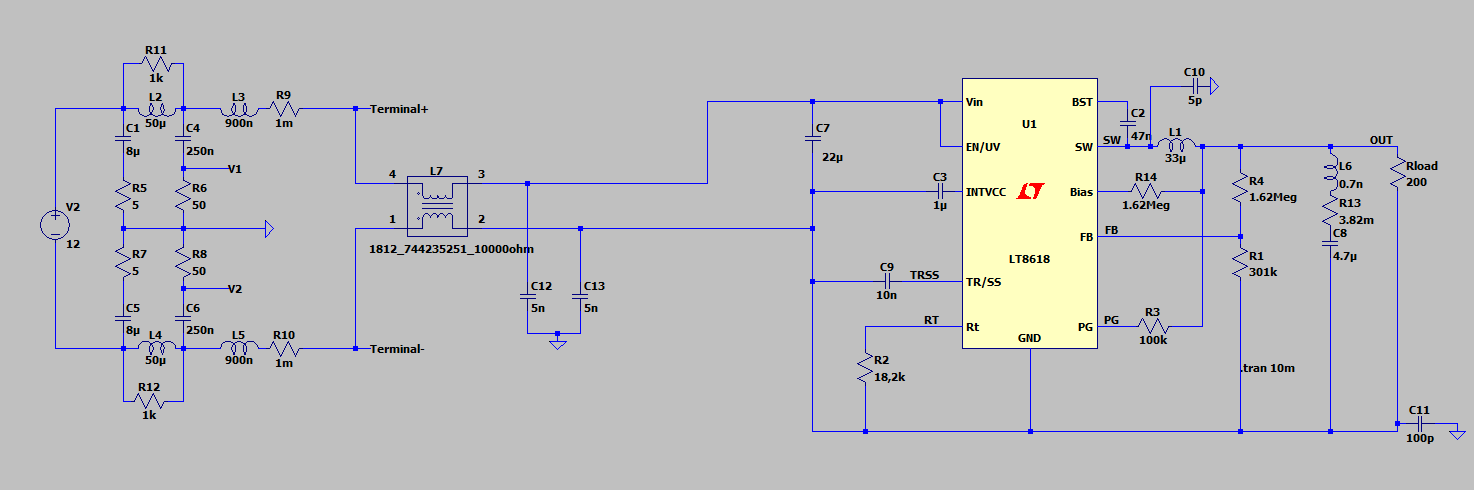
\includegraphics[width=0.8\textwidth]{img/schematic_cmc_x_cap_and_y_caps.png}
    \caption{Schematic: \GLS{acr:lisn} and buck converter with a rail to rail x-cap, a common mode choke and y-caps}
    \label{fig:cmc_x_cap_y_cap_schematic}
\end{figure}

\begin{figure}[htbp]
    \centering
    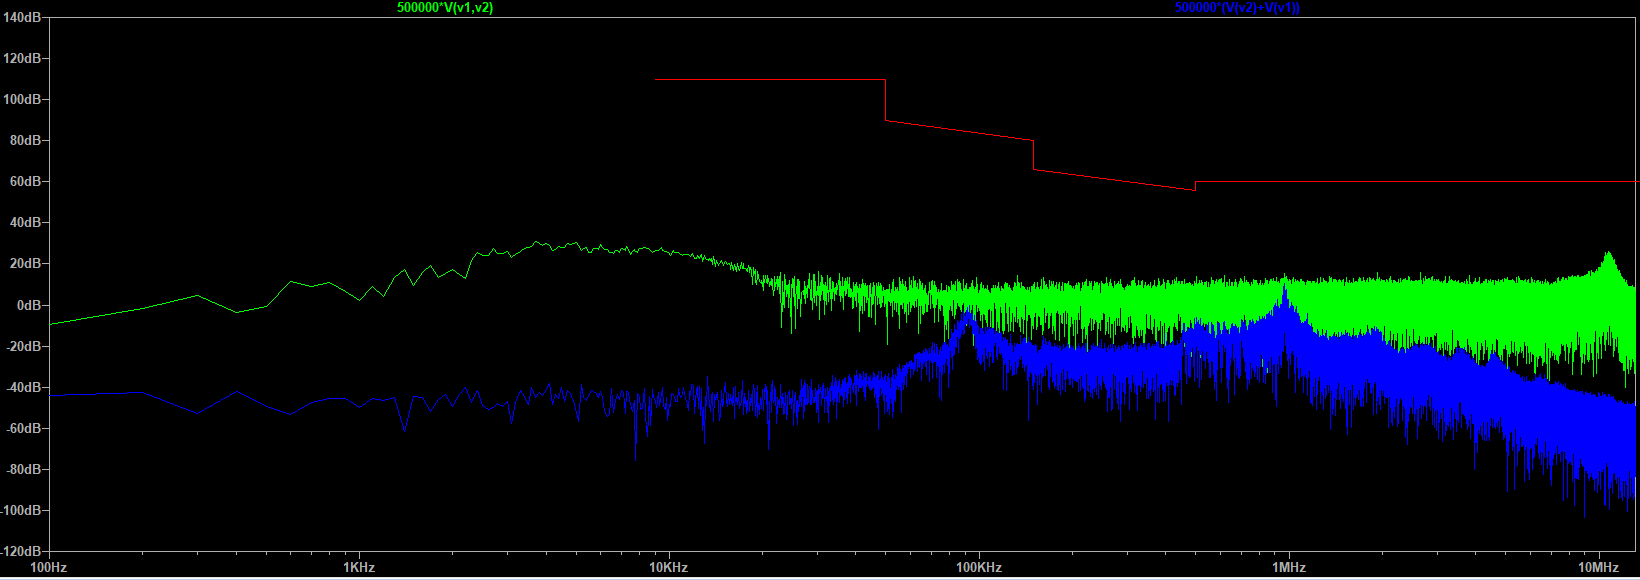
\includegraphics[width=0.8\textwidth]{img/emc_cmc_x_cap_and_y_caps.png}
    \caption{Conducted emissions of the buck converter with a rail to rail x-cap, a common mode choke and y-caps with \GLS{acr:dm} in green and \GLS{acr:cm} in blue, red line represents the conducted emissions limit}
    \label{fig:cmc_x_cap_y_cap_emc}
\end{figure}

\begin{figure}[htbp]
    \centering
    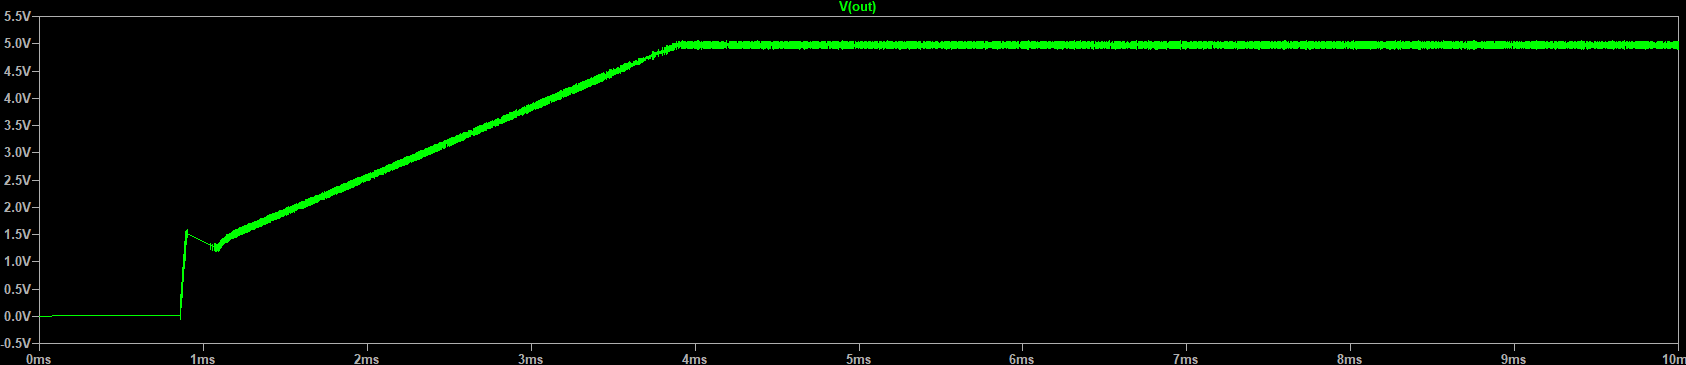
\includegraphics[width=0.8\textwidth]{img/vout_cmc_x_cap_and_y_caps.png}
    \caption{Output voltage of the buck converter with a rail to rail x-cap, a common mode choke and y-caps}
    \label{fig:cmc_x_cap_y_cap_vout}
\end{figure}




% EOF